\chapter{Developer documentation}
\label{ch:impl}

\section{Building the code}

There are currently two ways of building the code on Windows OS either with Visual Studio and using \textbf{vcpkg} as the package manager or with \textbf{MinGW} and manually building the packages (which I have deprecated but it's possible and I have put it in a separate branch).

First the following steps must be fulfilled to start developing (on windows):

\begin{itemize}
	\item Install \textbf{vcpkg} and add it to your path.
	\item Run the integrate install command so Visual Studio can detect it.
	\item Install CMake.
\end{itemize}

\subsection{Building with CMake}

To make it easier to download the required packages, a powershell script \texttt{install\_dependencies.ps1} is provided with the code which installs all the required dependencies.

Then the project can be built with CMake either by running \texttt{build\_for\_vs.ps1} script or by doing the following in the shell:
\lstset{caption={Building with CMake}, label=src:sh}
\begin{lstlisting}[language=bash]
mkdir build
cd build
cmake .. -G "Visual Studio 17 2022" -A x64 -DCMAKE_TOOLCHAIN_FILE=%PATH_TO_VCPKG%/scripts/buildsystems/vcpkg.cmake
\end{lstlisting}

You can replace generator with your compiler of liking, MinGW, for instance (if you have the packages installed). Replace the tool chain file path to your vcpkg path. 

CMake was chosen because of its cross-platform support. If, for instance, you want to build on linux and have the required packages then you can build using the same CMake file, in which case it will generate a Makefile instead of the VS solution.

\section{Design and the rendering pipeline}
This sections describes how the components fit together and in what order the things are rendered before proceeding to explain all steps in detail.

\subsection{The OpenGL Rendering Pipeline}
\begin{figure}[H]
    \centering
    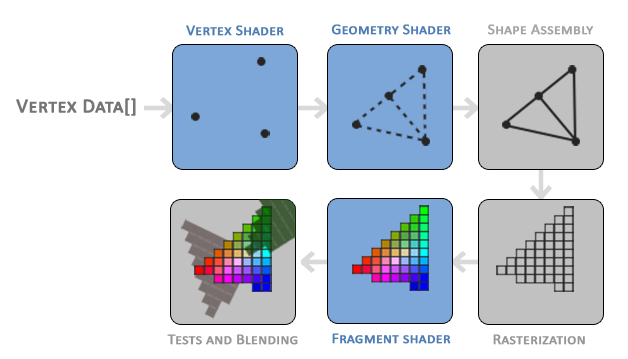
\includegraphics[width=0.75\textwidth]{images/opengl_pipeline.png}
    \caption{The OpenGL Pipeline} \cite{learnopengl}
    \label{fig:opengl_pipeline}
\end{figure}

First let's look at the OpenGL rendering pipeline in Figure~\ref{fig:opengl_pipeline}. The only procedures that we are concerned with at the moment are Vertex and Fragment shaders. Geometry shaders will be described at a later stage when they are needed.

\begin{definition}{Shaders}
	Shaders are programs that run on the GPU, there are various ways to send data to shaders. In the code, I mainly send data through vertex buffers or through uniforms. 
\end{definition}

Without going into too much depth, vertex shaders transform vertices from local space to normalized device coordinates and fragment shaders are used for choosing the colors (as depicted in the picture above).

\subsection{Vertex Shader Convention}
The code snippet below describes how a typical vertex shader looks like in the code:
\lstset{caption={Vertex shader convention}, label=src:vertex_convention}
\begin{lstlisting}[language=C]
layout (location = 0) in vec3 aPos;

uniform mat4 proj;
uniform mat4 view;
uniform mat4 model;

void main() {
	gl_Position = proj * view * model * vec4(aPos, 1.0);
}

\end{lstlisting}

In this document, I will be representing the projection matrix as $\mathbf{P}$, view as $\mathbf{V}$, and model as $\mathbf{M}$. In some vertex shaders there is also a local transformation matrix because I sometimes like to dissect the model matrix into two matrices the model and the local matrix, the former puts the object into the world space and the local transformation is responsible for any rotation or scaling.

\subsection{Shader loader}
To make it easier to load, compile and use shaders the engine comes with a Shader loading
class. The design of the shader loader/manager is inspired by the one on LearnOpenGL \cite{learnopengl}. This class is responsible for allocating and destructing the shaders. A different class is also defined specifically for loading Compute shaders which will be described later. However, the interface for using and setting the uniform variables is identical for both classes.

Uniform variables can easily be set using this shader class, as illustrated in the code snippet below (all such functions can be found in the header file):
\lstset{caption={Shader class usage example}, label=src:shader_usage}
\begin{lstlisting}[language=C++]
Shader myShader {"vertexSource.glsl", "fragmentSource.glsl"};
myShader.use();
myShader.setVec3("cameraPos", glm::vec3(0.0f));
\end{lstlisting}

\subsection{Mesh handling}
\label{subsec:mesh_handling}
In OpenGL the mesh data must be transferred to a \textbf{VBO (Vertex Buffer Object)} first and then the \textbf{VBO} must be bound to a \textbf{VAO (Vertex Array Object)}, instructions for how to parse the data in \textbf{VBO} must also be explicitly defined and optionally a drawing order of vertices can also be defined in a \textbf{EBO (Element Buffer Object)}. To make this simpler a \textbf{Mesh} class comes with the engine. This is also inspired by an implementation on LearnOpenGL \cite{learnopengl}. The figure below gives a rough UML of how the mesh class is structured.

\begin{figure}[H]
    \centering
    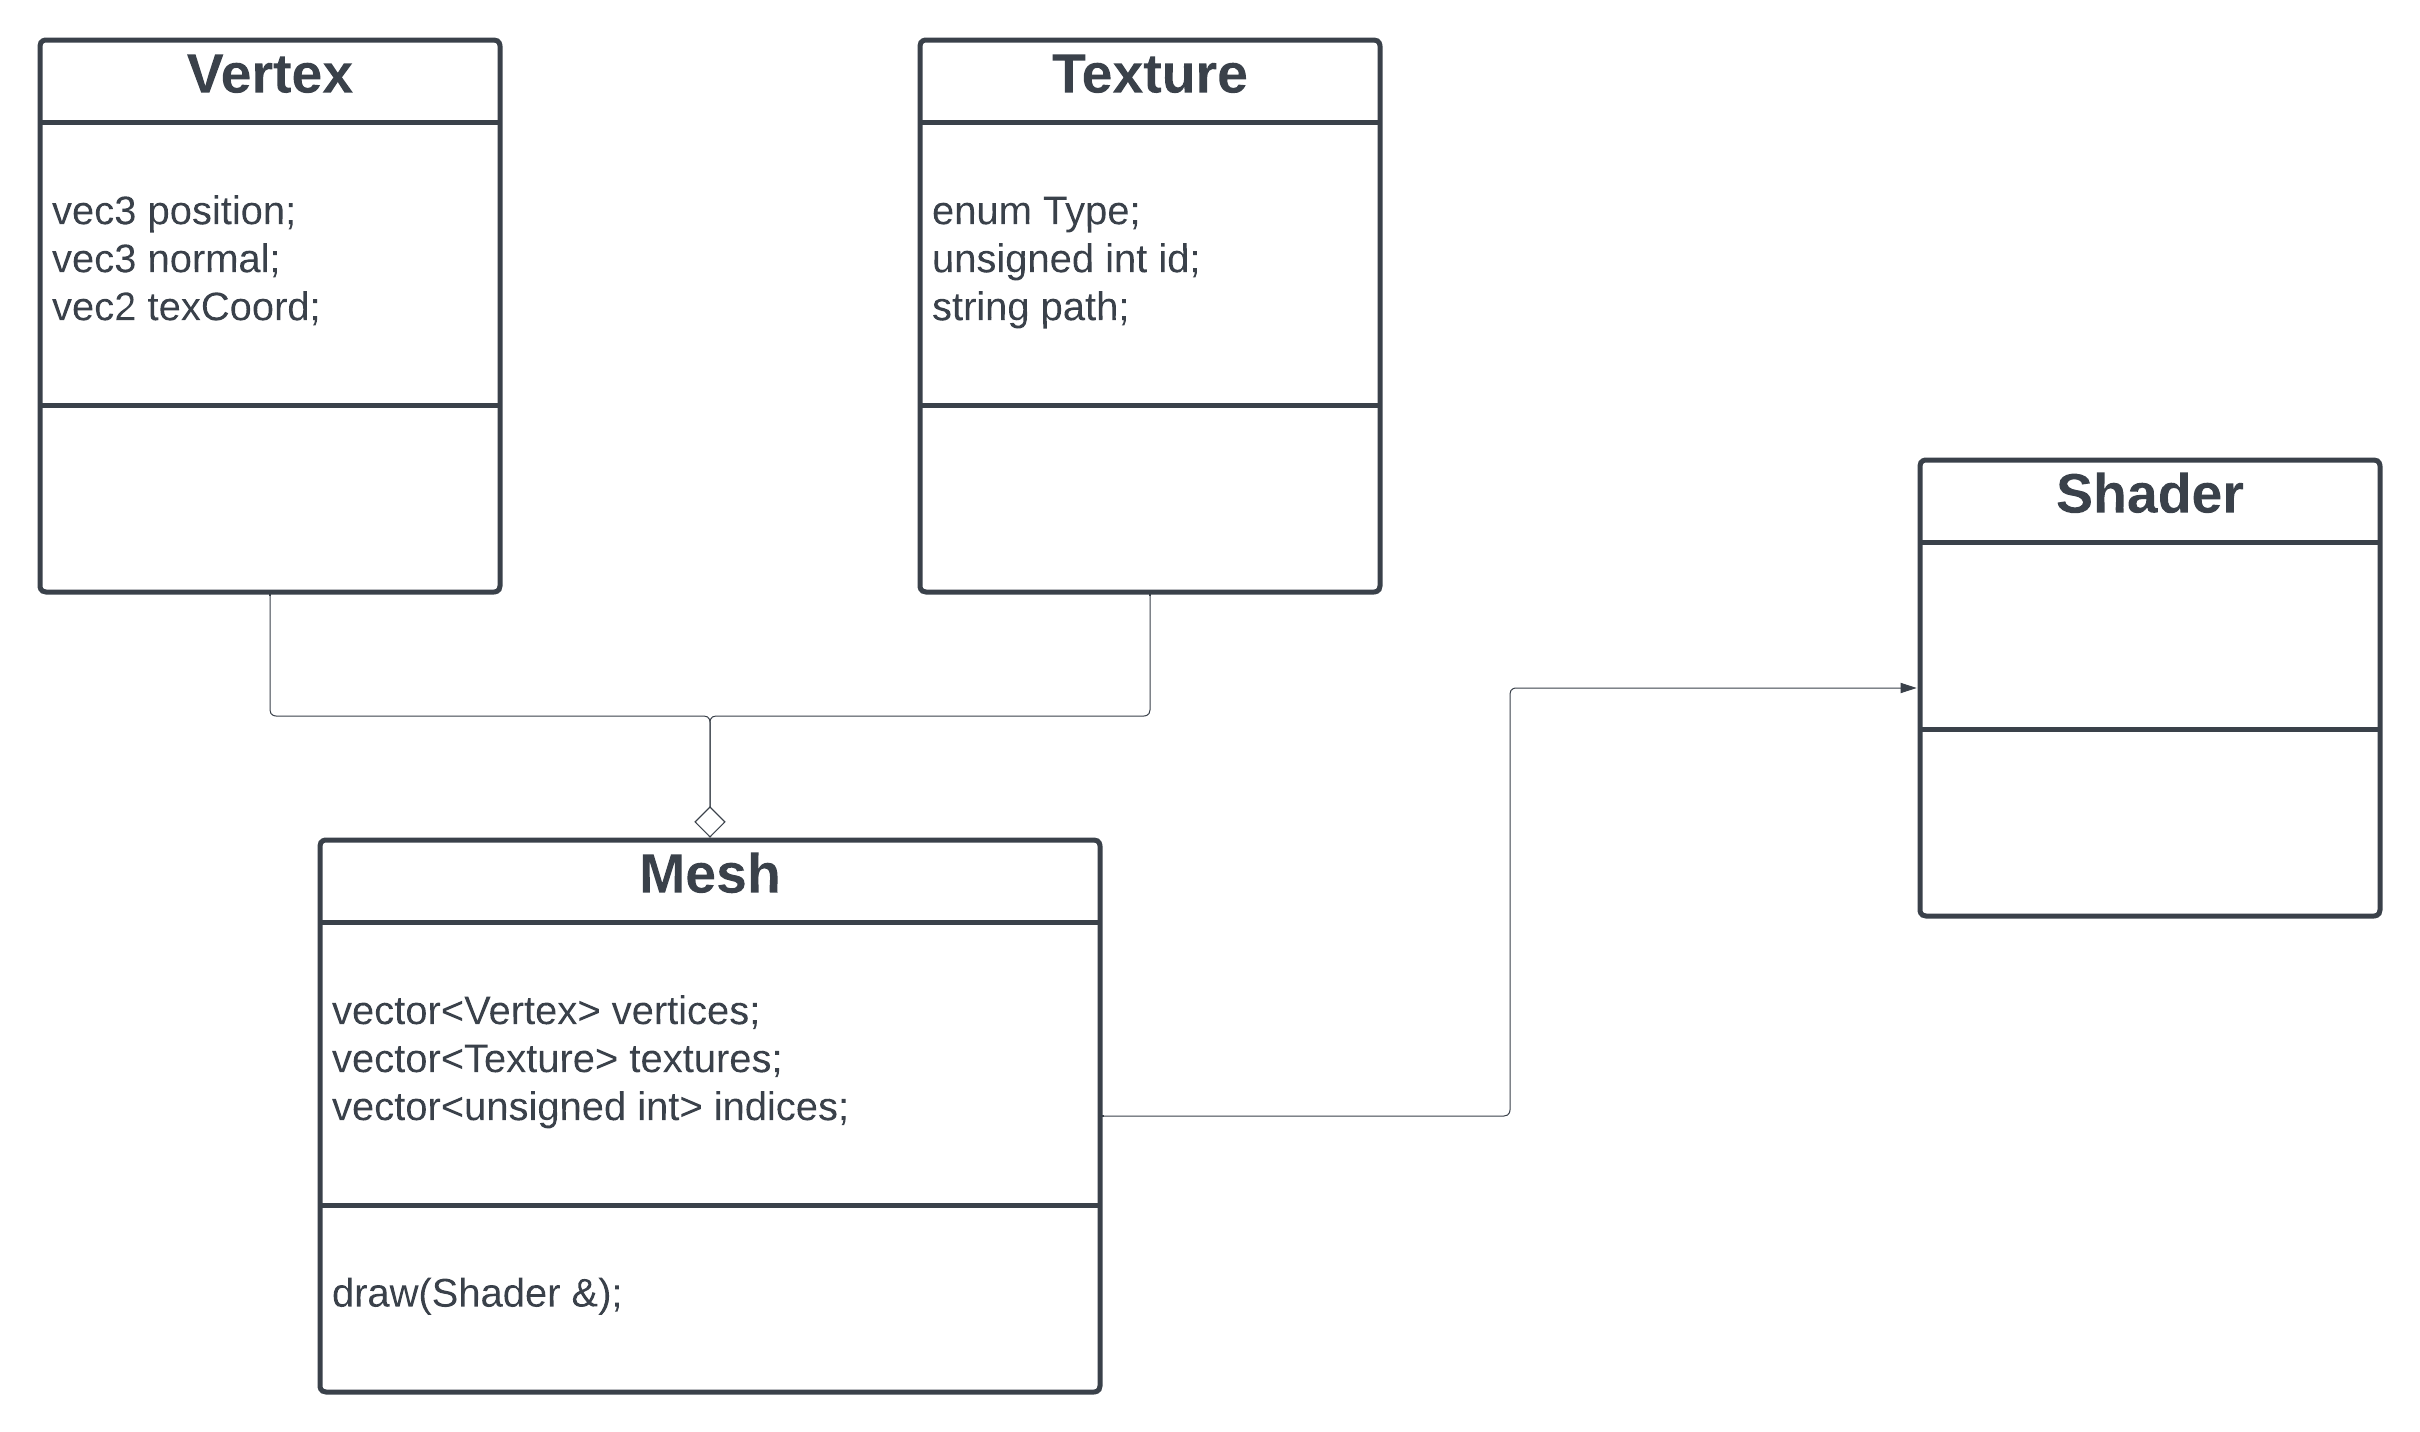
\includegraphics[width=0.75\textwidth]{images/mesh_uml.png}
    \caption{Mesh Class} \cite{learnopengl}
    \label{fig:mesh_uml}
\end{figure}

Meshes for 3d can be generated easily using a mapping $f (u, v)\rightarrow 
\langle x, y, z \rangle$. Some simple examples are given in \texttt{funcs.h} and \texttt{funcs.cpp}. For instance, a sphere can be generated using the function: $f (\theta, \phi) \rightarrow \langle \cos\theta\cos\phi, \sin\phi, \sin\theta\cos\phi \rangle$, where $\theta \in [0, 2\pi], \phi \in [-\frac{\pi}{2}, \frac{\pi}{2}]$. The normal vector for a sphere $\hat{n}$ is, of course, the same as $f (\theta, \phi)$. An implementation for generating the mesh of a torus is also given; a simple version of which can be derived by taking the parametric equation of a circle and translating it along, say, the x axis by $r\prime$: $C (\theta) = \langle r\cos\theta+r\prime, r\sin\theta, 0 \rangle$. If $\mathbf{R_y (\phi)}$ is the rotation around y axis then the torus is $f (\theta, \phi) = \mathbf{R_y( \phi)}C( \theta)$ where $\theta, \phi \in [0, 2\pi]$.


\subsection{Model loading}
The first implementation was done with a custom object file loader, however, it is infeasible to write a complete model loader that triangulates the vertices, supports multiple formats, and pares the texture files accurately. So, the decision to use \textbf{assimp} was made. The \textbf{Model} class is basically a wrapper around \textbf{assimp} functionality. This implementation was also motivated by the one provided on LearnOpenGL \cite{learnopengl}, however, contrary to that implementation this one is more optimized and handles the loading of materials more accurately.

The figure below can be used as a reference for understanding the code in the Model class.
\begin{figure}[H]
    \centering
    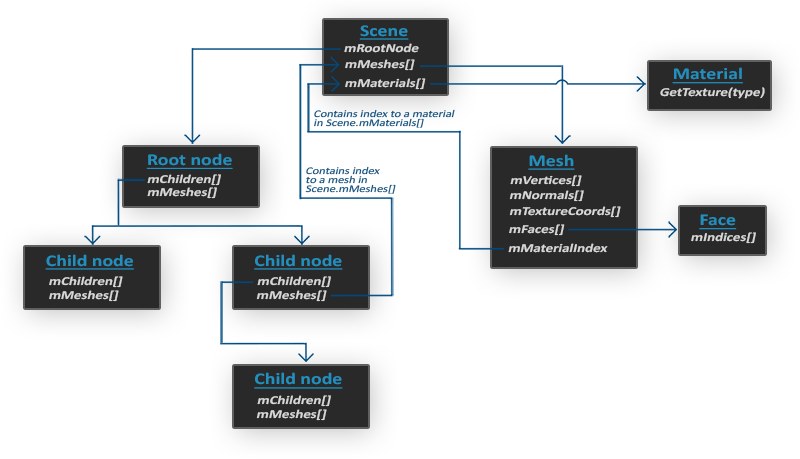
\includegraphics[width=0.75\textwidth]{images/assimp_structure.png}
    \caption{Assimp Structure} \cite{learnopengl}
    \label{fig:assimp_structure}
\end{figure}

A model can be thought of as a collection of meshes, so the rough UML diagram of the class below should make sense:
\begin{figure}[H]
    \centering
    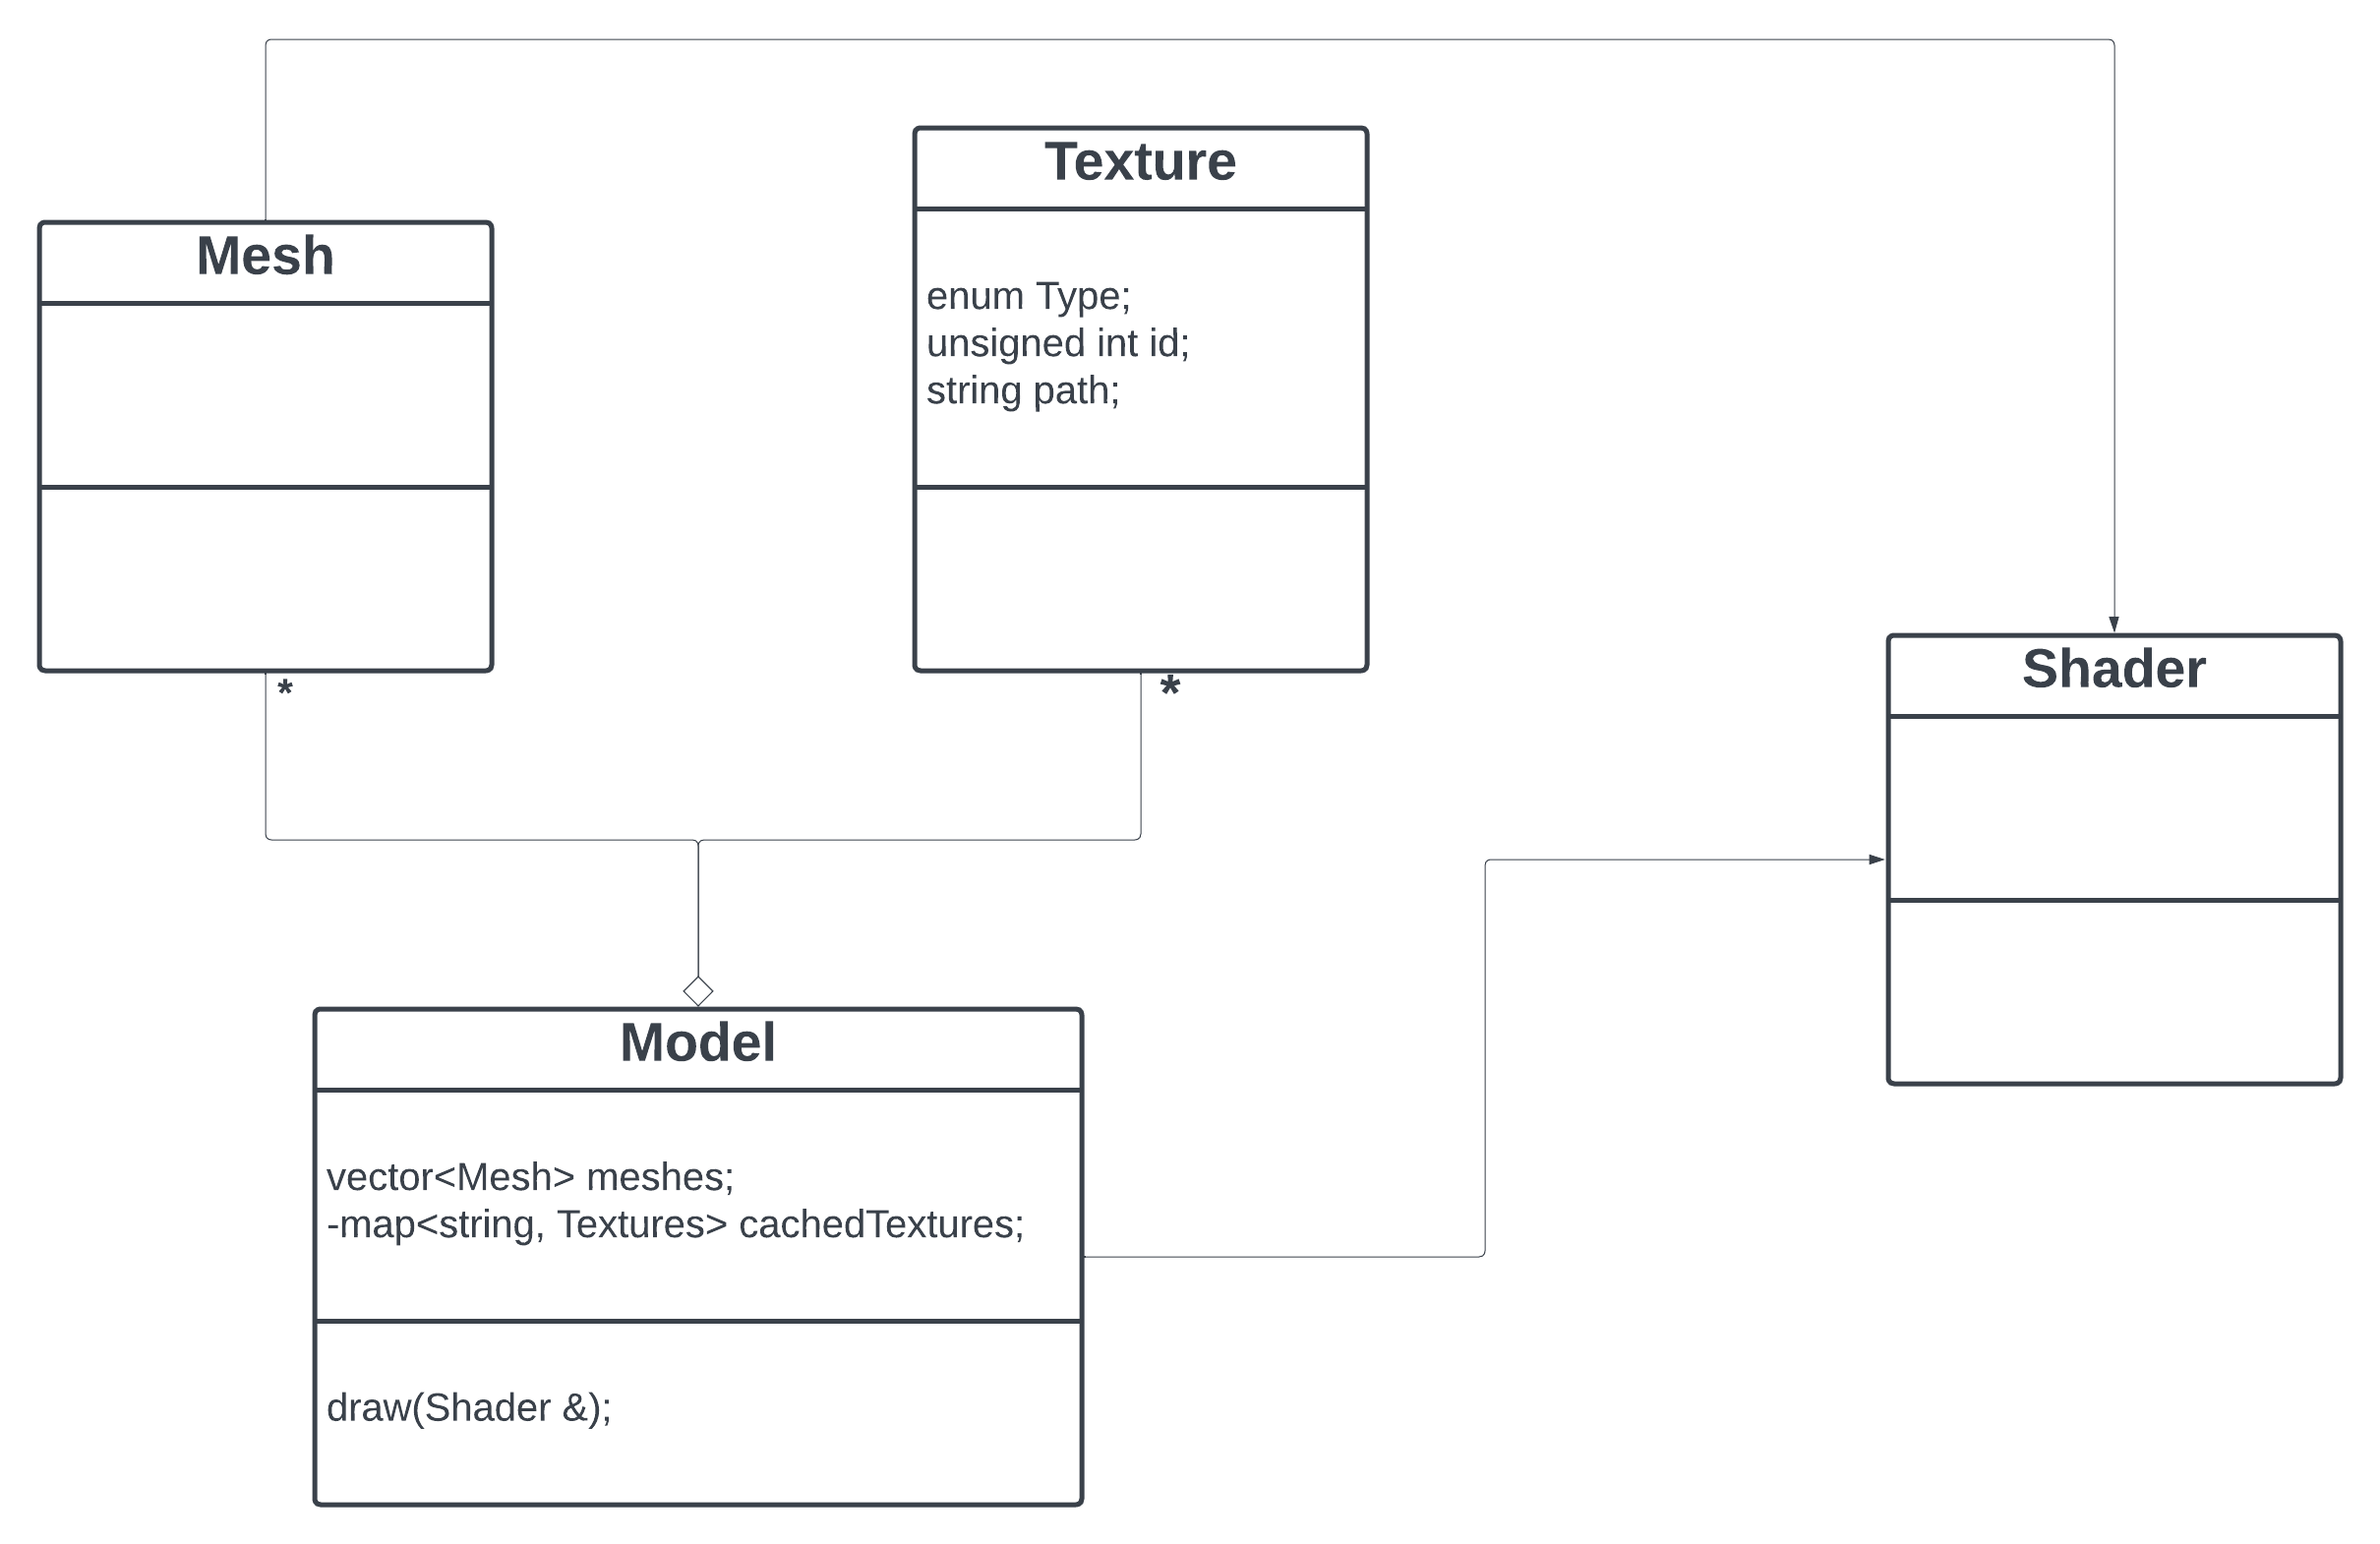
\includegraphics[width=0.5\textwidth]{images/model_uml.png}
    \caption{Model class UML}
    \label{fig:model_uml}
\end{figure}

Since models can have multiple diffuse and specular textures, they must be defined in the shaders in following convention. Diffuse textures must follow the following naming \textbf{texture\_diffuse[1..]}, specular textures must be named as \textbf{texture\_specular[1..]}.


\subsection{\texttt{Camera} class and the camera transform}

\begin{figure}[H]
    \centering
    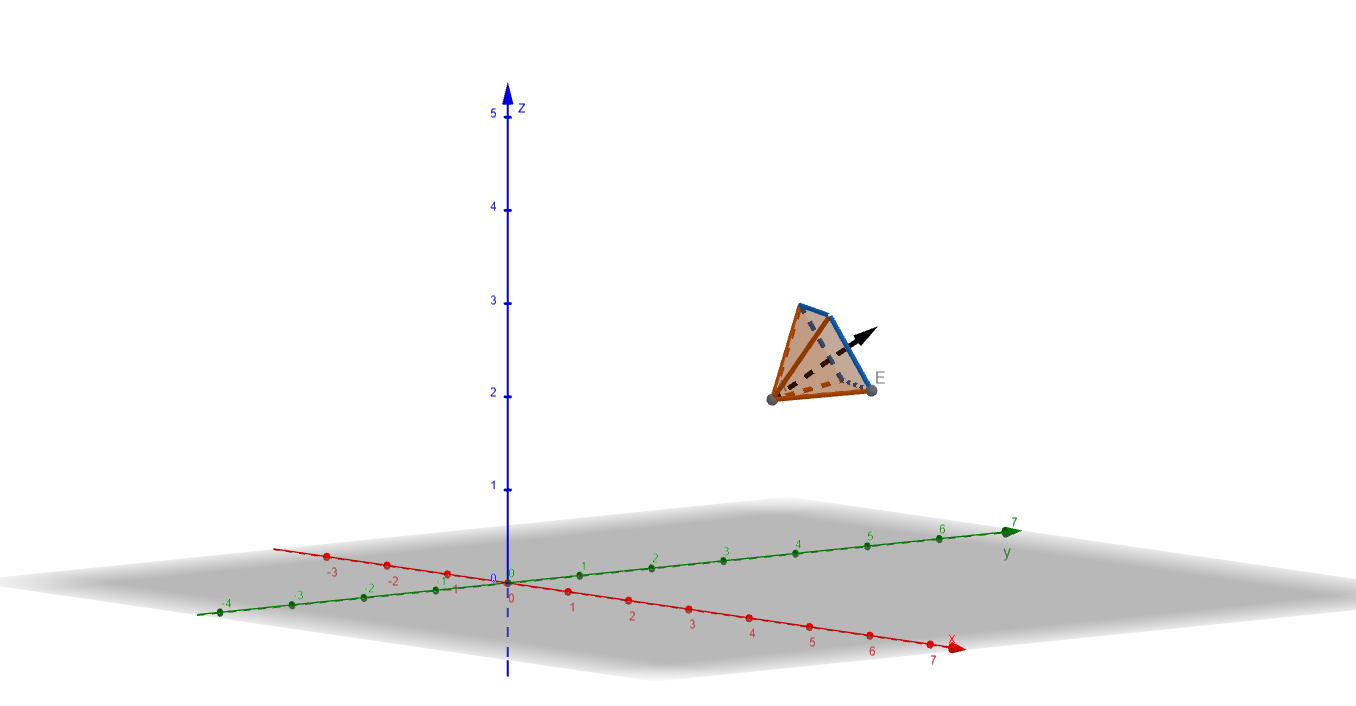
\includegraphics[width=0.75\textwidth]{images/camera_eg2.png}
    \caption{Simple Camera example}
    \label{fig:camera_eg}
\end{figure}

The camera can be imagined as a vector in the figure above. It sits at a point $\mathbf{p}$ looking in direction {$\mathbf{\hat{d}}$}. Contrary to some common implementations, which store a lookAt variable to store what point the camera is looking at, I only store the direction which can be dissected into two components: pitch (rotation around the $x-axis$), represented as $\phi$, and yaw (rotation around the $y-axis$) which is represented as $\theta$. Similar to what was done in the meshes section~\ref{subsec:mesh_handling}, it can be observed that these define a spherical coordinate system and we can get $\mathbf{\hat{d}}$ as follows: \begin{equation}\mathbf{\hat{d}} = \langle \cos\theta\cos\phi, \sin\phi, \sin\theta\cos\phi \rangle\end{equation}

However, the pitch is constrained to avoid distortions so, $\phi \in [-\frac{\pi}{4}, \frac{\pi}{4}]$. An absolute up direction vector is also defined for the camera which I will denote as $\hat{u}$ and $\hat{u}=\langle0, 1, 0\rangle$. The projection matrix works by assuming that the camera is looking in the negative $z-axis$ and is sitting at the origin. So $\mathbf{V}$ must be the matrix that puts the camera in this position. $\mathbf{V}$ must first translate the camera to the origin and then apply the inverse rotation of the current camera rotation.

If $\vec{p}$ is the position vector of the camera, then let $\mathbf{T_{-\overrightarrow{p}}}$ represent the translation matrix that translates by $-{\vec{p}}$.


The current rotation matrix of the camera can be obtained by getting the front (but flipped because the camera starts by looking in the negative $z$-axis), right, and up vectors of the camera:

\[
\hat{f} = \text{front} = -\hat{d}
\]
\[
\hat{r} = \text{right} = \hat{d} \times \hat{u}
\]
\[
\hat{a} = \text{up} = \hat{r} \times \hat{d}
\]

The rotation matrix is then:

\[
\mathbf{R} = \begin{bmatrix} 
\hat{r} & \hat{a} & \hat{f} 
\end{bmatrix}
\]

This can be imagined as where the $\hat{i}, \hat{j}, \hat{k}$ vectors land after the transformation.

We want the inverse of this matrix. Since this is an orthonormal matrix, the inverse is the transpose of the matrix:

\[
\mathbf{R^{-1}} = \mathbf{R}^T
\]

Thus, the final view matrix is:

\[
\mathbf{V} = \mathbf{R}^T \mathbf{T}_{-\mathbf{\overrightarrow{p}}}
\]


The \texttt{Camera} class in the code provides the above functionalities, and the view matrix can be easily obtained by calling the \texttt{camera.getView()} method.

\subsection{Audio Manager}

The engine includes an audio manager capable of playing 2D sounds. Currently, there is no implementation available for 3D audio playback. This component serves as a wrapper around the functionality provided by \textbf{OpenAL}. Audio files are loaded using \textbf{libsndfile}, and the engine currently supports only the \textbf{WAV} format.

The following code snippet demonstrates a basic usage example:

\lstset{caption={Audio Manager example}, label=src:audio_manager}
\begin{lstlisting}[language={C++}]
#include <audio_manager.h>
#include <iostream>

int main() 
{
    AudioManager audioMgr;
    audioMgr.play2d("soundfile.wav", /*loop*/ false);
    std::cin.get(); // prevent exiting
}
\end{lstlisting}


% TO DO: add text renderer, sprite renderer, explain homogenous coords if time permits.

\subsection{OpenGL Frame Buffer Objects and the \texttt{FrameBuffer} Class}

OpenGL provides Frame Buffer Objects (FBOs), which can be thought of as off-screen rendering targets—similar to virtual canvases or pseudo-windows that you can draw on. Instead of rendering directly to the screen, FBOs allow rendering to a texture or render buffer. This is particularly useful for post-processing effects, shadow mapping, and deferred rendering techniques.

The \texttt{FrameBuffer} class in the engine serves as a wrapper around OpenGL’s FBO functionality, simplifying the creation, configuration, usage, and memory management of frame buffer objects. It provides functionality to bind the FBO, with the option to clear it upon binding.

For simplicity, this implementation constructs the FBO using textures (rather than \textbf{Renderbuffer Objects}), as most parts of the engine require the ability to read from the framebuffer. A depth buffer is also included. These design choices can be modified in the future to support more flexible configurations.

A simple example is provided below:

\lstset{caption={Frame Buffer example}, label=src:frame_buffer}
\begin{lstlisting}[language={C++}]
#include <framebuffer.h>
#include <iostream>

int main() 
{
    // Ensure OpenGL context is active before using the FrameBuffer
    FrameBuffer frameBuffer;
    frameBuffer.bind();

    // All OpenGL draw calls will now render to the frame buffer
    // ...

    frameBuffer.unBind();

    // Access the color and depth texture IDs if needed
    GLuint colorTex = frameBuffer.textureId;
    GLuint depthTex = frameBuffer.depthTextureId;

    // Or, draw the FBO's content directly to the screen
    frameBuffer.draw(); 
}
\end{lstlisting}


\subsection{Architecture}

The UML diagram below represents a simplified architecture of the whole game and shows how the components connect to each other.

\begin{figure}[H]
    \centering
    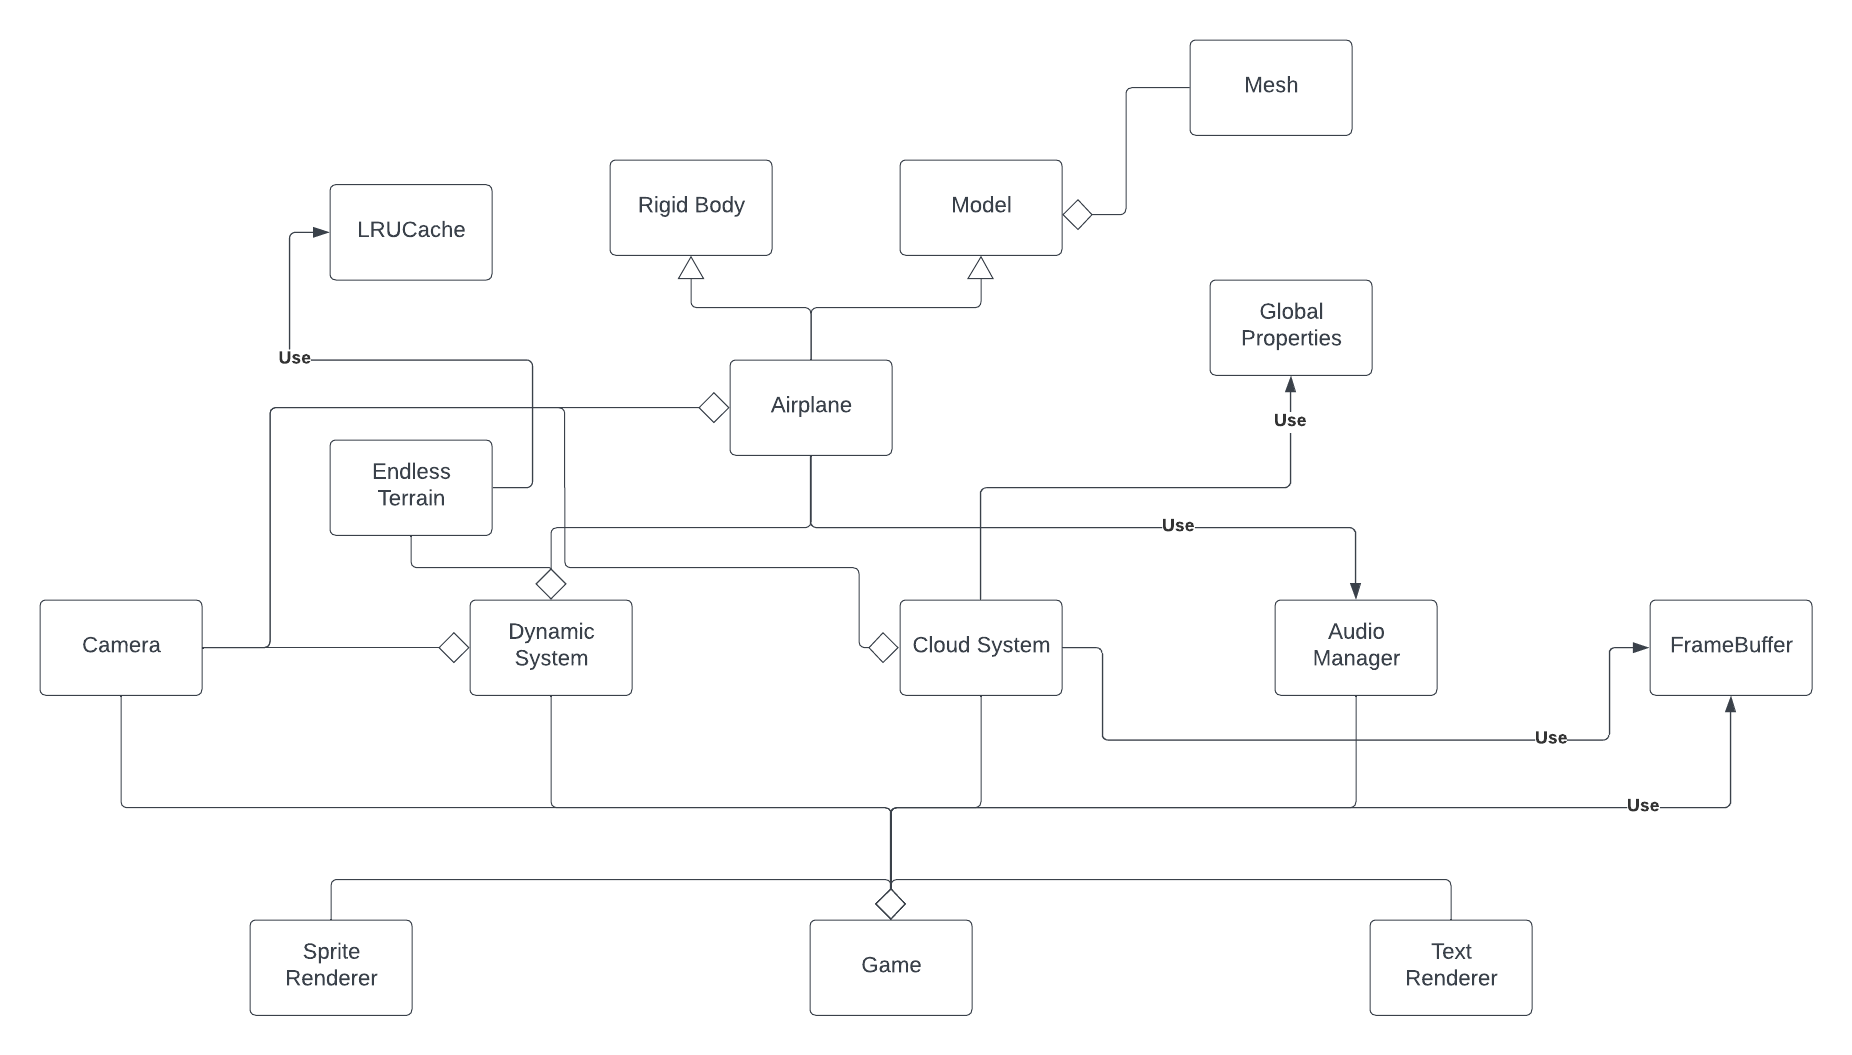
\includegraphics[width=1.0\textwidth]{images/architecture.png}
    \caption{Architecture}
    \label{fig:architecture}
\end{figure}


The main components i.e endless terrain, cloud system, rigid body, and airplane are explained the following sections.

\section{Procedural Terrain}

\subsection{Generating a chunk}

\begin{definition}[Chunk]
A \textit{chunk} refers to a rectangular mesh of predefined size, where each vertex contains height and normal vector information. Chunks serve as the basic building blocks for terrain generation and rendering.
\end{definition}

In most implementations where non-repetitive chunks are required, noise algorithms are commonly used. The algorithm I have chosen is \textbf{Perlin Noise} \cite{perlin2002improving}, which is implemented in \texttt{perlin.cpp}. Assuming, for now that we have some sort of a Perlin noise implementation available, a chunk that only has height data may be generated as simply as the following pseudo code shows:

\lstset{caption={Chunk generation}, label=src:chunk_gen}
\begin{lstlisting}[language=Python]
def generateChunkData(size, scale):
	chunkData = ChunkData(size, size)
	for i in range(size):
		for j in range(size):
			x = j * scale
			y = i * scale
			chunkData.height[i, j] = perlin(x, y)
	return chunkData
\end{lstlisting}

Next, we will explore how to extend this basic chunk with additional data such as normals and how to tile these chunks together for a continuous terrain. We will also dive into techniques such as Level of Detail (LOD) and early culling, which help improve performance and rendering efficiency in large terrains. First, let’s simplify Perlin Noise and look at how to calculate normals for our chunk data.


\subsection{Perlin Noise}

This section does not aim to provide a detailed theoretical explanation of the Perlin Noise algorithm. For a formal treatment, the reader is encouraged to refer to the original paper by Ken Perlin \cite{perlin2002improving}. For a more intuitive and visual explanation, see the video referenced in \cite{perlin_video}. 

Perlin Noise is a type of gradient noise that aims at generating smooth noise. If we, for instance, take a look at white noise where each pixel can be thought of as having a uniform probability of having a value between 0 and 1. The generated map as illustrated in Figure~\ref{fig:white_noise} looks completely random and this would never work as a height map as the height of a terrain is continuous.

\begin{figure}[H]
    \centering
    \begin{minipage}[t]{0.45\textwidth}
        \centering
        
\includegraphics[width=\textwidth]{images/white_noise.png}
        \caption{White Noise}
        \label{fig:white_noise}
    \end{minipage}
    \hfill
    \begin{minipage}[t]{0.45\textwidth}
        \centering
        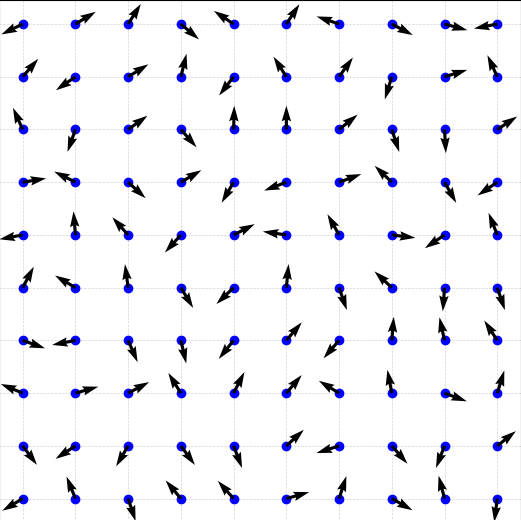
\includegraphics[width=\textwidth]{images/perlin_grid.png}
        \caption{Perlin Grid}
        \label{fig:perlin_grid}
    \end{minipage}
\end{figure}


Before looking into how Perlin noise works, let's define the \texttt{lerp} function.
\begin{definition}[\texttt{lerp}]
	Lerp is defined as :
	\[
		\texttt{lerp}(a, b, p) = a + p(b - a)
	\]
	% lerp(a, b, p) = $a + p(b-a)$
\end{definition}

% Perlin noise works by dividing a plane into a grid that has a random gradient vector assigned at each vertex as shown in Figure~\ref{fig:perlin_grid}. Let's just look at one box and call the point on the top left as $P_{tl}$ and vector associated with as $\vec{v_{tl}}$, we will label other points as $P_{tr}$, $P_{bl}$, $P_{br}$. If we take a point $U$ inside this box with coordinates ($U_x$, $U_y$), and ($u$, $v$) representing the fractional parts of ($U_x$, $U_y$) then the noise function as this point is evaluated as follows:\\
% Let $D_{tl}$ $=$ $P_{tl} - U$, $D_{tr}$, $D_{bl}$, $D_{br}$ are defined similarly. And Let $G_{tl} = \langle V_{tl}, D_{tl} \rangle$, $G_{tr}$, $G_{bl}$, $G_{br}$ are defined similarly.\\
% A step function $g(t)=6t^t-15t^4+10t^3$ is used for smoothing the values of $(u, v)$ and the noise is evaluated as 
% \begin{center}
% 	$noise(U_x, U_y)$ = \texttt{lerp}(\texttt{lerp}($G_{tl}$, $G_{tr}$, $g(u)$), \texttt{lerp}($G_{bl}$, $G_{br}$, $g(u)$), $g(v)$)
% \end{center}

Perlin noise works by dividing the plane into a grid, assigning a random gradient vector at each vertex, as shown in Figure~\ref{fig:perlin_grid}. Consider a single grid cell, and label the corners as follows:
\begin{itemize}
\item{Top-left: $P_{tl}$ with gradient $\vec{v}_{tl}$}
\item{Top-right: $P_{tr}$ with gradient $\vec{v}_{tr}$}
\item{Bottom-left: $P_{bl}$ with gradient $\vec{v}_{bl}$}
\item{Bottom-right: $P_{br}$ with gradient $\vec{v}_{br}$}
\end{itemize}

Let $U = (U_x, U_y)$ be a point inside the cell, and let $(u, v)$ be the fractional parts of $(U_x, U_y)$ relative to the cell.

Define direction vectors from each corner to $U$:
\[
\vec{d_{tl}} = U - P_{tl}, \quad \vec{d_{tr}} = U - P_{tr}, \quad \vec{d_{bl}} = U - P_{bl}, \quad \vec{d_{br}} = U - P_{br}
\]

Next, compute the dot products:
\[
G_{tl} = \langle \vec{v}_{tl}, \vec{d_{tl}} \rangle, \quad G_{tr} = \langle \vec{v}_{tr}, \vec{d_{tr}} \rangle, \quad G_{bl} = \langle \vec{v}_{bl}, \vec{d_{bl}} \rangle, \quad G_{br} = \langle \vec{v}_{br}, \vec{d_{br}} \rangle
\]

A smoothing function is used to interpolate values:
\[
g(t) = 6t^5 - 15t^4 + 10t^3
\]

Finally, the noise value at point $U$ is computed using bilinear interpolation:
\[
\texttt{noise}(U_x, U_y) = \texttt{lerp}(\texttt{lerp}(G_{tl}, G_{tr}, g(u)), \texttt{lerp}(G_{bl}, G_{br}, g(u)), g(v))
\]

\subsection{Calculating normals}
In general, given a parametric surface $f(u, v)$ it is possible to obtain surface normal at specific points by the following formula: 
\[ \hat{n} = \frac{\frac{\partial{f}}{\partial{u}} \times \frac{\partial{f}}{\partial{v}}}
{\|\frac{\partial{f}}{\partial{u}} \times \frac{\partial{f}}{\partial{v}}\|}
\]
One way to imagine this is to see that $\frac{\partial{f}}{\partial{u}}$ and $\frac{\partial{f}}{\partial{v}}$ span the plane that is tangent to the surface, so their cross product gives the normal vector. For a more mathematically sound argument, you can refer to Paul's Online Notes \cite{dawkins_parametric_surfaces}.
In our case the mesh is made up of triangles as seen in Figure~\ref{fig:mesh_eg} but we can still calculate surface normals using cross products.

\begin{figure}[H]
    \centering
    \begin{minipage}[t]{0.45\textwidth}
        \centering
        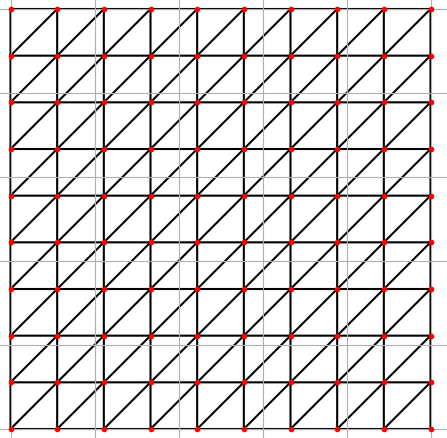
\includegraphics[width=\textwidth]{images/mesh_eg.png}
        \caption{Mesh}
        \label{fig:mesh_eg}
    \end{minipage}
    \hfill
    \begin{minipage}[t]{0.45\textwidth}
        \centering
        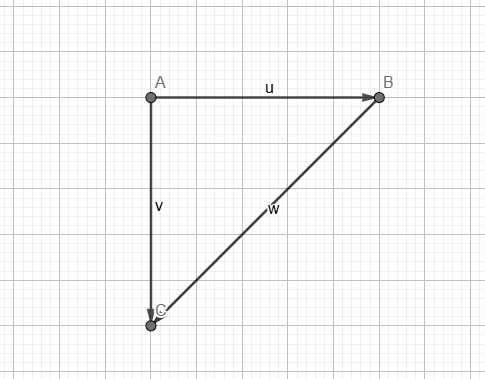
\includegraphics[width=\textwidth]{images/normal_eg.png}
        \caption{Calculating normal of a triangle}
        \label{fig:normal_eg}
    \end{minipage}
\end{figure}

As Figure~\ref{fig:normal_eg} shows we can calculate the normal at vertex \textbf{A} by calculating $u \times v$ (or $v \times u$ this direction is usually checked empirically) where $u$ and $v$ are the vectors of the triangle. This figure is 2d but it can be imagined the all 3 points \textbf{A}, \textbf{B}, and \textbf{C} are at different heights but the math works the same. 

\begin{figure}[H]
    \centering
    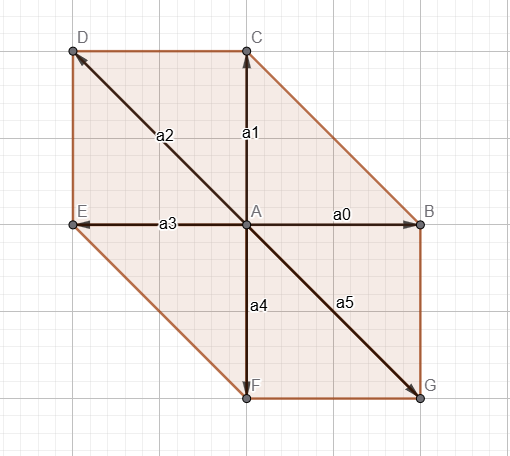
\includegraphics[width=0.5\textwidth]{images/normal_calc.png}
    \caption{Normal Calculation}
    \label{fig:normal_calc}
\end{figure}


However, vertex \textbf{A} is in multiple triangles. Figure~\ref{fig:normal_calc} shows my approach for calculating the normals. I take the 4 vertices around \textbf{A} let's call them $\mathbf{a_0}...\mathbf{a_3}$ in either counterclockwise or clockwise ordering (depending on which way defines the vectors in the up direction). Then the normal vector can be calculated as follows:
\[
\vec{n} = \frac{1}{4}\sum_{i=0}^{i=3}{(\mathbf{a_i}-\mathbf{A}) \times (\mathbf{a_{(i+1) \bmod 4}} - \mathbf{A})}
\]
Which is the average of the the normal vectors for each of the 4 triangles. For this to work correctly, you must ensure the vertices are in the correct ordering.

As the picture above suggests, this breaks down at the edges of the mesh. To circumvent this issue, I pad the mesh with extra set of vertices that is used just for the calculation of normals.

So, the pseudocode with normals looks something like this:
\lstset{caption={Chunk generation Part 2}, label=src:chunk_gen2}
\begin{lstlisting}[language=Python]
def generateChunkData(size, scale):
	heightData = Matrix(size + 2, size + 2) // matrix with num rows, cols = size + 2
	for i in range(size + 2):
		for j in range(size + 2):
			x = j * scale
			y = i * scale
			heightData[i, j] = noise(x, y)
	
	chunkData = ChunkData(size, size)
	for i in range(1, size):
		for j in range(1, size):
			vs = getNeighbors(i, j) //should return list of 4  neighbors in the correct order
			vertex = Vector(i, heightData[i, j] ,j)
			normal = Vector(0, 0, 0)
			for k in range(4):
				a = vs[k]
				b = vs[(k + 1) % 4]
				normal += cross(a-vertex, b-vertex)
			mag = normal.magnitude()
			if mag != 0:
				normal /= mag
			chunkData[i-1, j-1].height = heightData[i, j]
			chunkData[i-1, j-1].normal = normal			
	return chunkData
\end{lstlisting}

\subsection{Geometry Shaders and verifying the correctness of the normals}

It still needs to be checked if the normals calculated are actually correct and one way of doing that is to visualize them using geometry shaders. A tutorial for which can be found on LearnOpenGL \cite{learnopengl}. The \texttt{Shader} class provided with the engine takes an optional third argument -the geometry shader source file- so, integrating it into the existing system is easy.  

A geometry shader can take primitives as input (a triangle in our case) and can output primitives. For each vertex of the triangle we can emit a line with two vertices one at the original vertex, the other one in the direction of the normal but scaled by some constant $\alpha$.

The scene must be rendered twice once with the normal shader and again with the geometry shader. Figure~\ref{fig:terrain_normals} was obtained using this pipeline:
\begin{figure}[H]
    \centering
    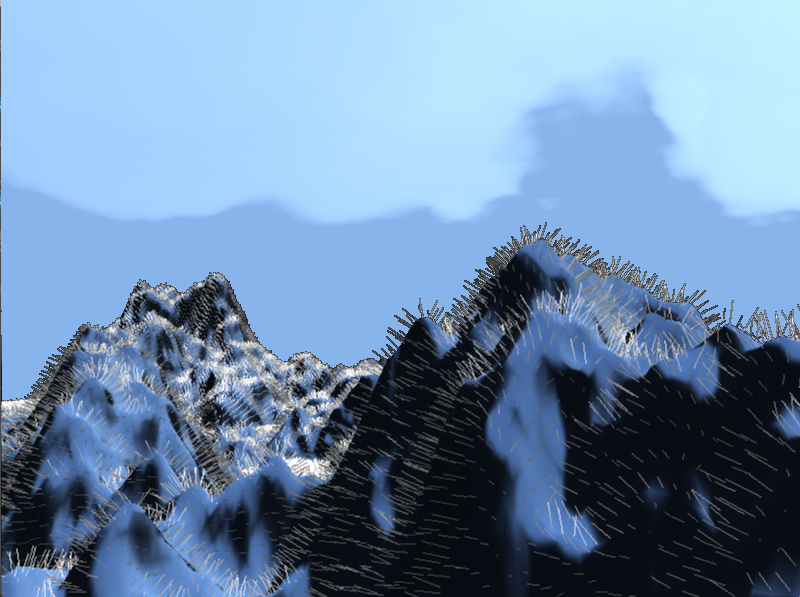
\includegraphics[width=0.5\textwidth]{images/normals.png}
    \caption{Visualizing Terrain Normals}
    \label{fig:terrain_normals}
\end{figure}


\subsection{Tiling the chunks}
Once we have the chunk generation function above it's not too hard to tile them. Since Perlin Noise accepts $(x, y)$ as the arguments we just need to make sure when going from one chunk to the next we give the correct coordinates to Perlin Noise. To do this, I extended the chunk generation function to accept one more argument: its \texttt{center}, using this it calculates the noise as it previously did from its top left corner but this time shifted by the \texttt{center} coordinates.

The following pseudocode explains how it is done:
\lstset{caption={Chunk generation Part 3}, label=src:chunk_gen3}
\begin{lstlisting}[language=Python]
def generateChunkData(size, center, scale):
	heightData = Matrix(size + 2, size + 2) // matrix with num rows, cols = size + 2
	tlX = (size - 1)/-2.0 //top left x
	tlY = (size - 1)/2.0 //top left y
	for i in range(-1, size + 1):
		for j in range(-1, size + 1):
			x = (center.x + tlX + j) * scale
			y = (center.y + tlY - i) * scale
			heightData[i, j] = noise(x, y)
	
	//rest remains same
\end{lstlisting}

If the loop started from \texttt{0}, then \texttt{center.x + tlX} would give the x-coordinate of the current chunk. However, at index $(0, 0)$, we actually want to sample from the previous chunk's coordinate space due to the padding added for normal calculation. Therefore, the loop must begin at \texttt{-1} to correctly align the noise sampling with the padded grid.

\subsection{Level Of Detail (LOD)}

It's important for a better FPS to render the chunks near the player at a higher level of detail than those that are further away. LOD can be thought of in this case as the number of vertices in a given area or volume.

To do this I first create a mesh and then further lower resolution meshes are created by skipping some vertices in the original mesh such that the first and the last vertices are not skipped because the mesh must extend from and to the same points. This begs the question then what should be the size of the original mesh? Consider a 1d mesh of size 10 as the picture below~\ref{fig:one_d} illustrates. We cannot skip every 2nd vertex because then we will have $\langle 0, 2, 4, 6, 8 \rangle$ and the last 9th vertex would be skipped.

\begin{figure}[H]
    \centering
    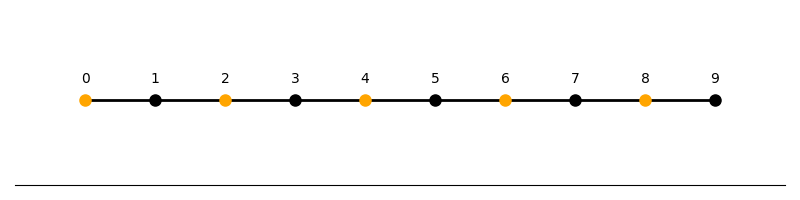
\includegraphics[width=0.75\textwidth]{images/one_d.png}
    \caption{1D mesh}
    \label{fig:one_d}
\end{figure}

So, if $k$ is the skip factor and $s$ is the size of the mesh, then for us to be able to create a mesh, $k$ must divide $s-1$. We need to find $s$ such that $s-1$ has a lot of divisors, and a commonly chosen number is \textbf{$241$} since every number from $1$ to $6$ divides $240$ so we can create a mesh that has $\frac{1}{6}$ of the vertices in the original mesh.

A common approach for this is to generate these meshes on the fly as a function of the distance from the player's coordinates. However, I found this method to not match my FPS goals. So, what I do instead is create the 6 LOD meshes beforehand and give the corresponding mesh its height and normal data through a texture. Height and normal data are stored in a texture, where both of them are packed into a \texttt{vec4} using the red, green, blue, and alpha channels. Each mesh then simply samples from this texture to obtain terrain shape and lighting information.

Unlike traditional LOD systems that generate meshes at runtime based on camera distance, this approach precomputes multiple LOD meshes and uses texture data to drive the final geometry. This reduces runtime computation and improves FPS stability at the cost of some memory overhead.

The image~\ref{fig:lod_terrain} below illustrates how \textbf{LOD} meshes look like in practice.

\begin{figure}[H]
    \centering
    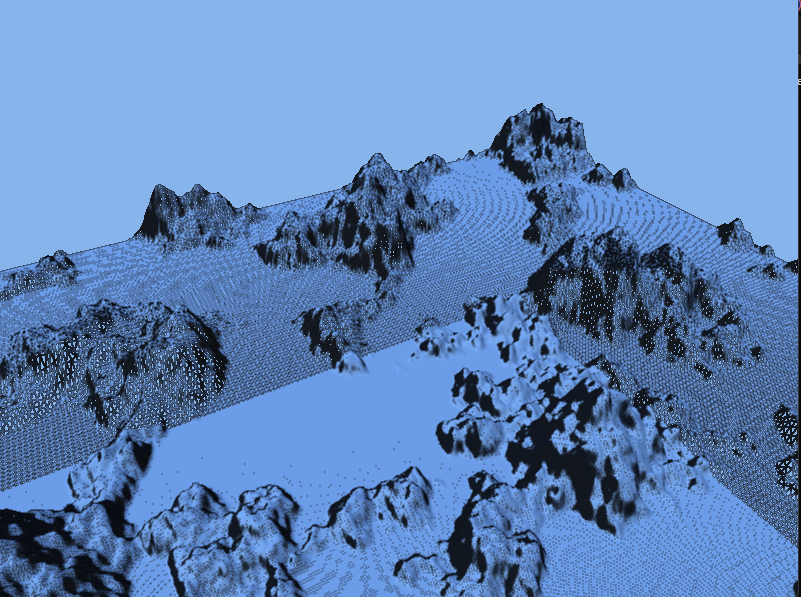
\includegraphics[width=0.5\textwidth]{images/LOD.png}
    \caption{Visualizing LOD Terrain}
    \label{fig:lod_terrain}
\end{figure}

\subsection{Multithreading}
It is not feasible to draw and generate new chunks on the same thread; for instance, we may need to generate 9 chunks at once, which would block the main render loop and drop the frame rate. To avoid this, a new thread is dispatched for generating data for each chunk. Since the meshes are already pre-generated (as discussed in the LOD section), the data needed is just height and normals.
Figure~\ref{fig:chunk_pipeline} illustrates this pipeline.

\begin{figure}[H]
    \centering
    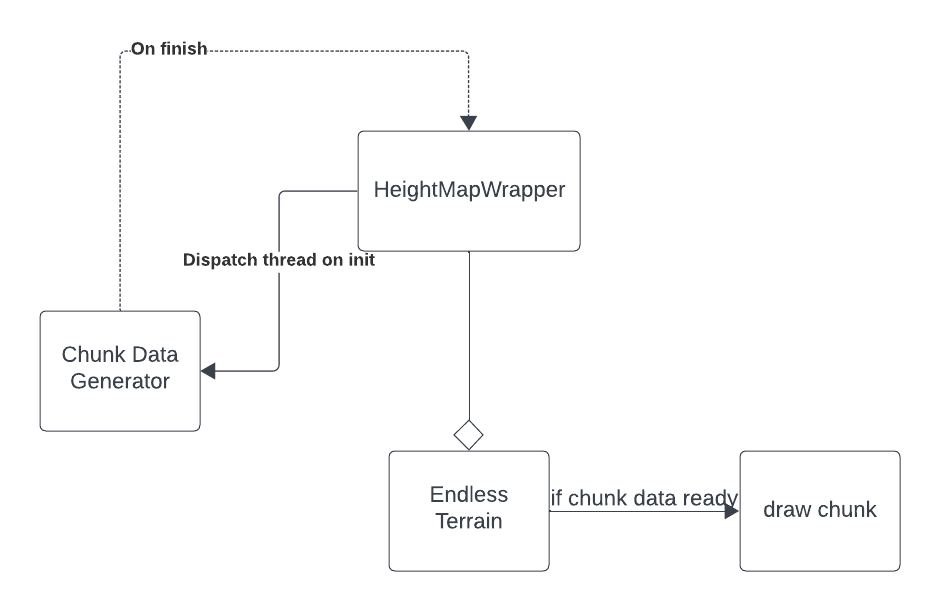
\includegraphics[width=0.75\textwidth]{images/chunk_process.png}
    \caption{Chunk Drawing Pipeline}
    \label{fig:chunk_pipeline}
\end{figure}

The \texttt{EndlessTerrain} class only draws a chunk once its data is ready. When a chunk is needed, it initializes a \texttt{HeightMapWrapper} instance, passing in the chunk center. This wrapper then launches a new thread to request height and normal data from the \texttt{ChunkDataGenerator} (which is just a simple function in the code). Once the data is computed, it is returned via a callback function, completing the pipeline.
\\
\textbf{\large IMPORTANT:}\\
It is crucial to note that OpenGL operates strictly on a single thread—all OpenGL commands must be issued from the same thread that initialized the OpenGL context. Because of this, the \texttt{HeightMapWrapper} class handles all computation on the CPU first. Once the data is available (from the background thread), it schedules OpenGL commands to upload the data to the GPU as a texture, all on the main thread.

\subsection{Caching and the \texttt{LRUCache} class}
Imagine we generate 9 chunks around the player for a single frame, to avoid re-generating them in the next one we must cache them. A straightforward solution would be to use a hashmap where the key is the center of the chunk and the value is the corresponding height map. However, this approach leads to an unbounded cache, which can eventually exhaust system memory.

To solve this, I used the \texttt{LRUCache} class that comes with the engine—a bounded version of the classic hashmap. If the maximum cache size is $n$ and a new key is inserted when the cache is full, the least recently used (LRU) key is evicted to make space.

Since LRUCache is a well-known data structure, its full implementation details are omitted. However, figure~\ref{fig:lru_cache} illustrates its core design using a doubly linked list, which should provide enough insight into how the code operates.

\begin{figure}[H]
    \centering
    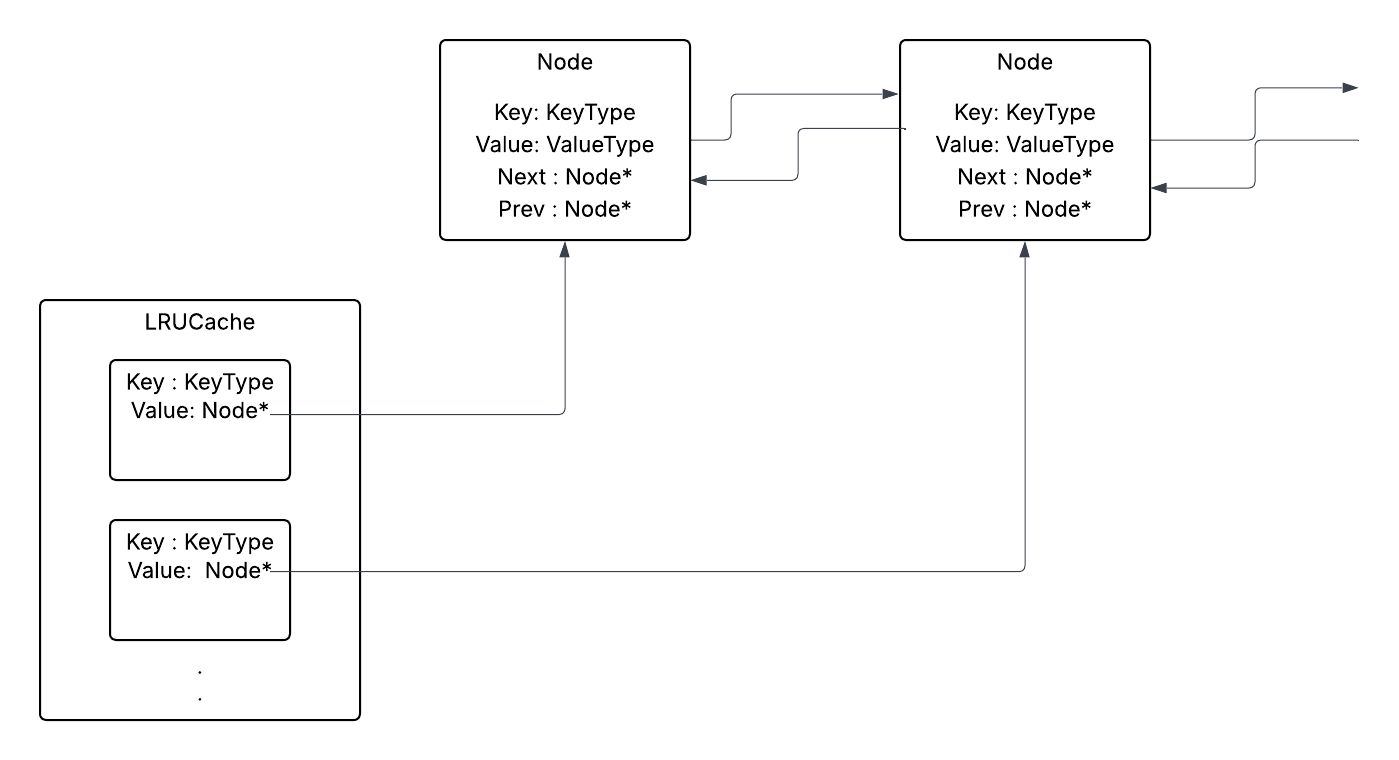
\includegraphics[width=0.75\textwidth]{images/lru_cache.png}
    \caption{LRUCache design}
    \label{fig:lru_cache}
\end{figure}

\subsection{Early Culling}
Notice that the methods above issue generate and draw commands for chunks that are not in the view frustum of the player. This introduces an overhead that can be easily avoided. For instance, the chunks that are behind the player can be omitted. To address this, I use a simple directional culling approach: Say, $\vec{d}$ is the direction of the camera and $\mathbf{P}$ is its position, when we are generating the $i_{th}$ chunk with center $\mathbf{C_i}$ around the player, let $\vec{v} = \mathbf{P}-\mathbf{C_i}$ be the direction of the chunk. We only generate data for the chunk if $\langle \vec{d}, \vec{v} \rangle > 0$ that is, both of those vectors point in the same direction. Note that if $\vec{v}$ is 2 dimensional that $\vec{d}$ must be projected on to the plane. In the code provided, $\mathbf{P}$ is projected onto the $x-z$ plane and so is $\vec{d}$.

\textbf{Result:} This optimization led to a significant performance gain—FPS improved, and memory usage dropped from around 500 MB to around 100MB.


\section{Volumetric Clouds}
This section explains my implementation of volumetric clouds. Before delving into the details, I would like to acknowledge the resources that were instrumental in my work and would like to thank the online community: \cite{sebestianlague2019} \cite{shadertoy2013} \cite{guerrillagames2025nubis} \cite{reinder2018} \cite{fredrik} \cite{gamedevnet2015horizonzerodawn} \cite{palenik2016volumetricclouds} \cite{maxime2023} \cite{engel2016gpupro7}.
\subsection{Ray Marching}

Before delving into cloud rendering, we must understand the basics of ray marching. Ray marching is a technique where we trace rays for each pixel on the screen. Unlike ray tracing, which requires information about polygonal geometry, ray marching only requires access to a signed distance function ($\text{sdf}$). 

A signed distance function for an object $O$ and a point $P$ returns the distance from $P$ to the nearest point on $O$'s surface. It is:
\begin{itemize}
\item{positive if $P$ is outside the object}
\item{negative if $P$ is inside}
\item{and zero if $P$ lies on the surface}
\end{itemize}

For example, the signed distance function for a sphere is:
\[
\text{sdf}(p) = \|p - c\| - r
\]
where $c$ is the center and $r$ is the radius of the sphere.

A ray is defined by its origin $P$ and direction $\vec{d}$. We represent it as a function of time:
\[
R(t) = P + \vec{d}t
\]

If there are multiple objects in the scene, the scene’s overall signed distance function is defined as:
\[
\text{sdf}_{\text{world}}(P) = \min_{\text{objects}} \text{sdf}_{\text{object}}(P)
\]

Ray marching works by advancing the ray by the distance given by the $\text{sdf}$ at each step, as illustrated in the following code snippet:

\lstset{caption={Basic Ray Marching}, label=src:basic_raymarch}
\begin{lstlisting}[language=C]
int MAX_STEPS = 1000;
float MIN_DIST = 1e-4;
float MAX_DIST_TRAVEL = 1e3;

vec3 trace(Ray r) // returns light info
{
    vec3 currentPos = r.pos;
    float totalDistTraveled = 0.0;

    for (int i = 0; i < MAX_STEPS; ++i)
    {
        currentPos = r.pos + r.direction * totalDistTraveled;
        float dist = sdf_world(currentPos);

        if (dist < 0) break;

        else if (dist < MIN_DIST) {
            // do light calculation
            return /* light info */;
        }

        if (totalDistTraveled > MAX_DIST_TRAVEL) break;

        totalDistTraveled += dist;
    }
    return vec3(0.0);
}
\end{lstlisting}

The illustration in Figure~\ref{fig:raymarching_eg} shows this process in 2D, which can be interpreted as a top-down view of a 3D scene.

\begin{figure}[H]
    \centering
    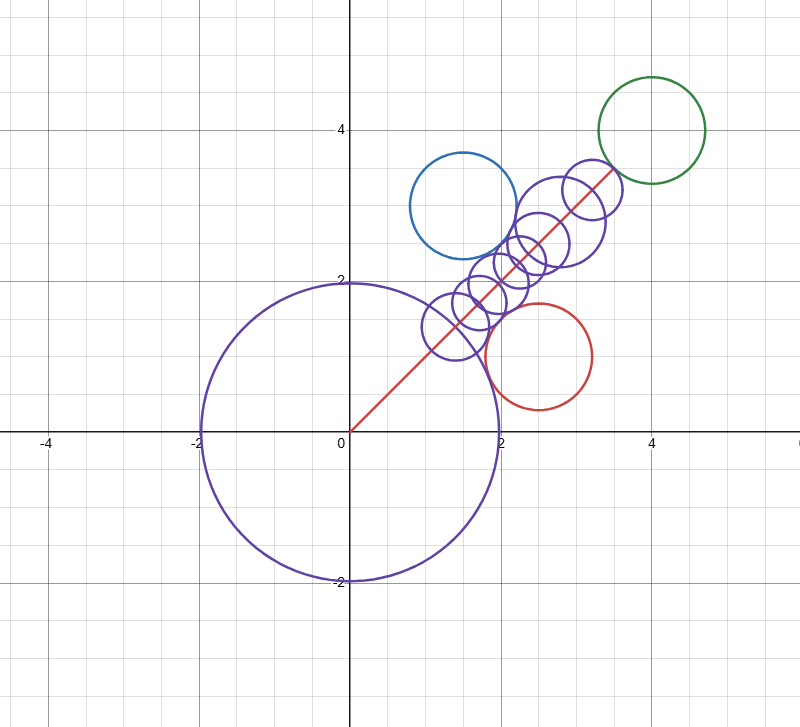
\includegraphics[width=0.5\textwidth]{images/raymarching_eg.png}
    \caption{Ray marching example}
    \label{fig:raymarching_eg}
\end{figure}

When $\text{sdf}(p) = 0$, the surface near point $p$ can be locally approximated by the equation $\text{sdf}(p) = 0$. For an implicit surface $f(x, y, z) = c$ (which can be thought of as a equipotential surface in 3D or level curve in 2D), the surface normal is given by the gradient:
\[
\nabla f = \left\langle \frac{\partial f}{\partial x}, \frac{\partial f}{\partial y}, \frac{\partial f}{\partial z} \right\rangle
\]

Using a symmetric finite difference approximation:
\[
\frac{df}{dx} \approx \frac{f(x + h) - f(x - h)}{2h}
\]

we can approximate the normal at point $p$ from the signed distance function as:
\[
\vec{n} = \left\langle 
\text{sdf}(p + h\hat{i}) - \text{sdf}(p - h\hat{i}),
\text{sdf}(p + h\hat{j}) - \text{sdf}(p - h\hat{j}),
\text{sdf}(p + h\hat{k}) - \text{sdf}(p - h\hat{k})
\right\rangle
\]

This normal vector is then used in lighting calculations.\footnote{This reasoning was derived independently (so it's more intuitive than rigorous) but is consistent with standard SDF-based normal estimation techniques used in ray marching.}

\subsection{Ray Marching for rendering volumes}
For rendering volumetric surfaces like clouds instead of using $sdf$ functions a fixed step size $\delta$ is chosen and the ray is moved forward by this step size at each step. At each point $P$ in space density is sampled and the rendering is done based on how much density was observed, how much light passed through and so on. More details are in the following section but first for clouds my implementation makes a rectangular area in the sky where the clouds can be, this is a axis aligned bounding box (AABB). First, a check is done to see if the ray intersects this box; if yes, only then is the ray marched through the box.
Next, we derive the intersection of a ray with AABB. Remember that a ray is given as $R(T) = P + \vec{d}t$. An axis aligned box can be defined by its top left coordinates and bottom right coordinates denoted as $b_{min}$, $b_{max}$.
\[
b_{min} \le P + \vec{d}t \le b_{max}
\]
\[
b_{min} - P \le \vec{d}t \le b_{max} - P
\]
which gives 3 inequalities:
\[
\frac{(b_{min, x} - P_x)}{\vec{d}_x} \le t \le \frac{(b_{max, x} - P_x)}{\vec{d}_x}
\]
\[
\frac{(b_{min, y} - P_y)}{\vec{d}_y} \le t \le \frac{(b_{max, y} - P_y)}{\vec{d}_y}
\]
\[
\frac{(b_{min, z} - P_z)}{\vec{d}_z} \le t \le \frac{(b_{max, z} - P_z)}{\vec{d}_z}
\]

if $[t_{min}, t_{max}]$ is the intersection of those intervals, then the ray intersects the box if $t_{max} \ge t_{min}$ with $t_{min}$ being the nearest point of intersection and $t_{max}$ being the furthest. If the point is inside the box then clearly, $t_{min} < 0$ in this case we return $t_{max}$ as the intersection $t$. if $t_{max} < 0$, the box must be behind the ray, so there is no intersection.

\subsection{Worley Noise}
